% !TEX TS-program = pdflatex
%\documentclass[draftcls, onecolumn, journal]{IEEEtran}
\documentclass[journal]{IEEEtran}
%\documentclass[a4paper,11pt]{article}
%\usepackage{fullpage}

%\renewcommand{\baselinestretch}{1.9}
\usepackage[hidelinks]{hyperref}
\usepackage{graphicx}
\usepackage{color}
\usepackage{amsmath}
\usepackage{subcaption}
\usepackage{algorithmicx}
\usepackage{algorithm}
\usepackage{algpseudocodex}
\usepackage{cleveref}
\usepackage{diagbox}
%\usepackage{multicol}
%\usepackage{cite}
\usepackage[
style=ieee,
sorting=ynt
]{biblatex}
\graphicspath{images/}
\addbibresource{sources.bib}


\newcommand{\argmax}[1]{\underset{#1}{\operatorname{arg}\,\operatorname{max}}\;}

%\bibliographystyle{IEEEtran}

%%%%%%%%%%%%%%%%%%%%%%%%%%%%%%%%%%%%%%%%%%%%%%%%%%%%%%%%%%%%%%%%%%%%%%
\title{Fan-Beam Computerized Tomography Simulation \newline Algebraic Reconstruction Techniques}

\author{Kutay Ugurlu}

%%%%%%%%%%%%%%%%%%%%%%%%%%%%%%%%%%%%%%%%%%%%%%%%%%%%%%%%%%%%%%%%%%%%%%
\begin{document}
%\renewcommand{\baselinestretch}{1.6}

\maketitle

\begin{abstract}This project report demonstrates the implementation of Fan Beam Computerized Tomography simulation with Algebraic Reconstruction Techniques. A couple of experiments considering different design parameters and algorithms are conducted to compare the performances of these techniques. The effect of these parameters is inspected and discussed comparatively in both quantitative and qualitative manner.
%\textit{Keywords:} Inverse electrocardiography, electrocacardiographic imaging, statistical estimation, Bayesian estimation, Kalman filter.
\end{abstract}
\begin{IEEEkeywords}
	Imaging, medical imaging, X-Ray computerized tomography, image reconstruction, algebraic reconstruction technique(ART)
\end{IEEEkeywords}

\section{Introduction} \label{sec:intro}
The purpose of this project report is to demonstrate the different reconstruction algorithms and their relative performances. This project report consists of \nameref{sec:theory}, \nameref{sec:implementation}, \nameref{sec:results} and \nameref{sec:discuss} sections. The second section introduces the technical background for the Algebraic Reconstruction Technique algorithms.  

\subsection{History}
The history of X-Ray Computerized Tomography can be dated back to 1917, when an Austrian mathematician called Johann Radon invented an algorithm, referred to as Radon transform today, on how to calculate line integrals in a two-dimensional section. The idea of computed tomography was developed in 1967 and was first used in a medical setting was in 1971 \cite{richmond2004sir}, by Godfrey Hounsfield. The device was tested at
James Ambrose’s department at Atkinson Morley Hospital in Wimbledon. This first model did not include a computer, instead the waves was written on a magnetic tape of the device EMI Scanner CT1010 in Figure \ref{fig:CT1010}. It was in 1973 that commercial CT scanners were available to the public. \cite{CTHist}

\begin{figure}[h]
\centering
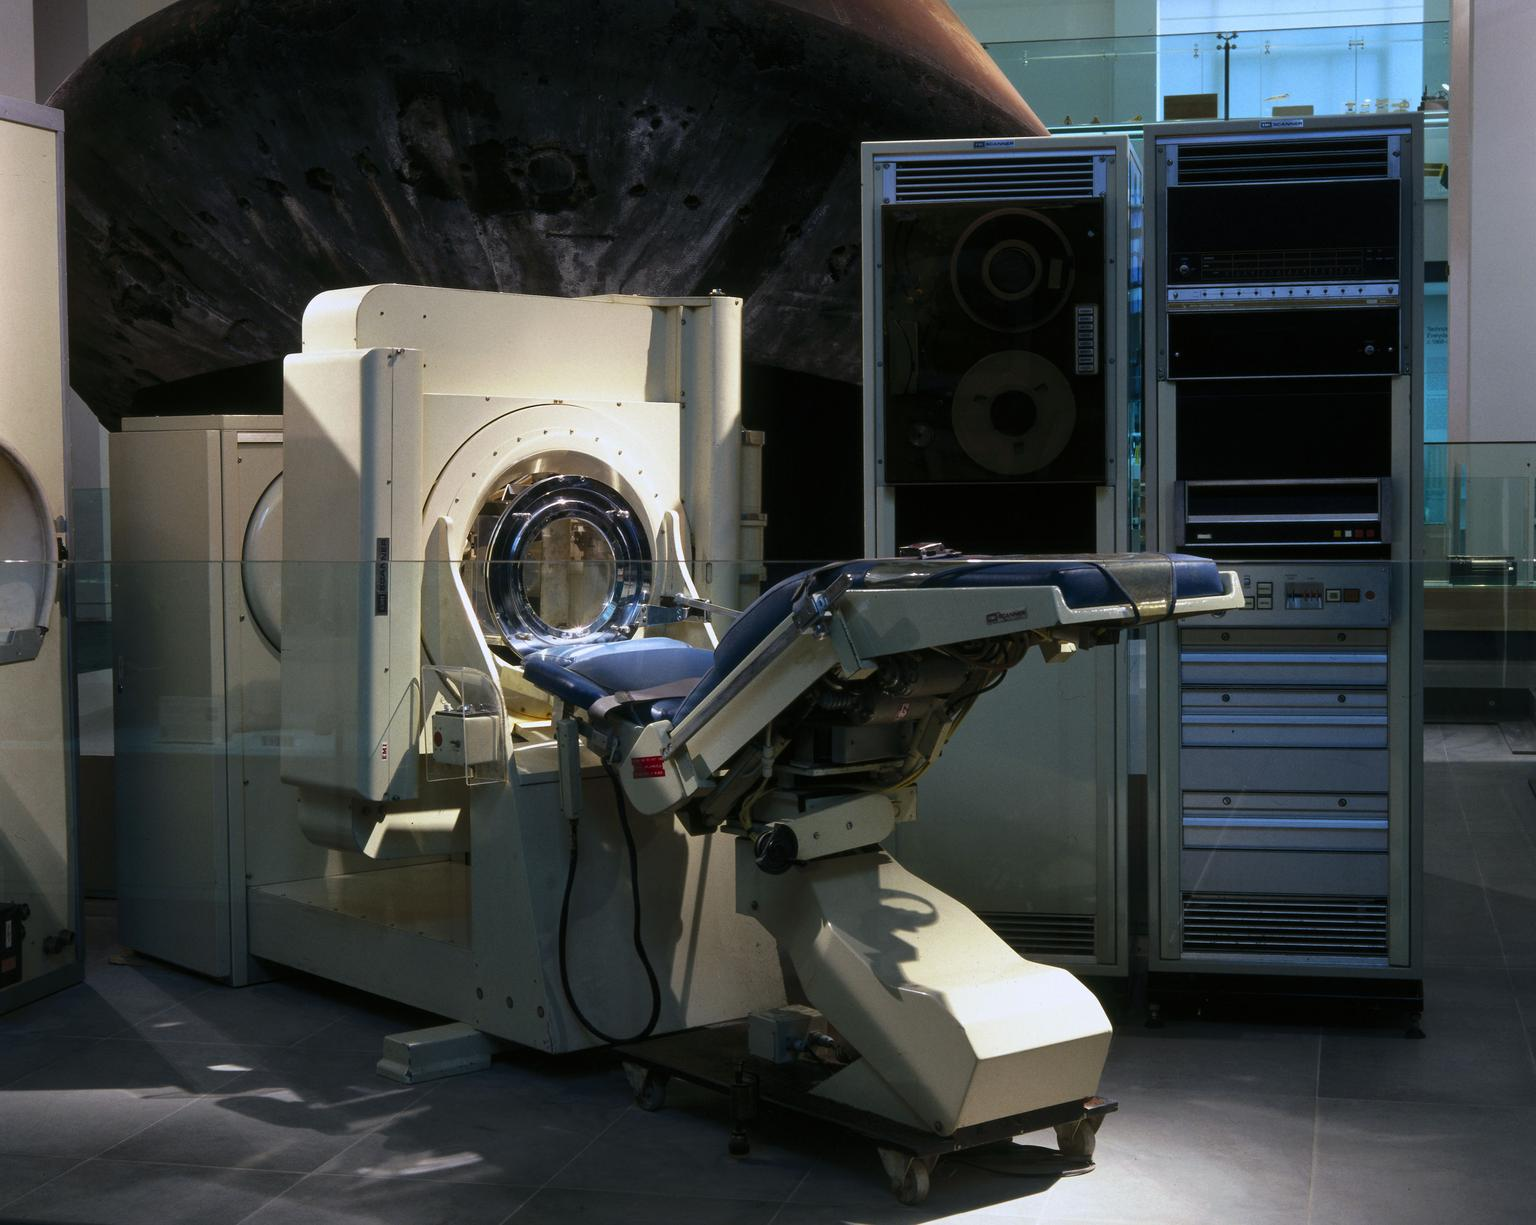
\includegraphics[width=0.4\textwidth, height=0.2\textwidth]{images/CT.jpg}
\caption{First EMI Scanner \cite{emict}}\label{fig:CT1010}
\end{figure}

\vfill{\null}

\section{Theory} \label{sec:theory}
\subsection{X-Ray Attenuation}
In X-ray tomography, images are modelled as attenuation coefficient distributions which is a measure of how much X-ray beams are attenuated when they propagate through an object. This problem can be modeled as in Eqn. \ref{eq:radon3d} for an arbitrary object.
\begin{equation} 
	I_{measured} = I_0 e^{-\iiint\limits_{object}\mu(x,y,z)dxdydz}
	\label{eq:radon3d}
\end{equation}
When the object to be imaged is two-dimensional or can be reduced to a two-dimensional slice, Eqn \ref{eq:radon3d} reduces to Eqn \ref{eq:radon2d}:
\begin{equation}
	I_{measured} = I_0 e^{-\iint\limits_{slice}\mu(x,y)dxdy}
	\label{eq:radon2d}
\end{equation}
\subsection{Radon Transform}
Radon Transform computes the line integrals along the objects to obtain projections along an arbitrary angle $\theta$ for an arbitrary beam t, using the formula given in Eqn. \ref{eq:radongeneral}.
\begin{equation}
	p_{\theta}(t) = \iint\limits_{-\infty}^{\ \ \ \infty}\mu(x,y)\delta(xcos(\theta)+ysin(\theta)-t)dxdy
	\label{eq:radongeneral}
\end{equation}
This equation models the X-ray beams as parallel lines through the object. In a more practical scenario, the X-ray source is modelled as a point source and beams are projected from source to the object in fan beam shape, due to the equiangular spaced discrete detector locations. This modelling can be achieved by introducing geometric transformation between projection variables. 

\begin{figure}[h]
\centering
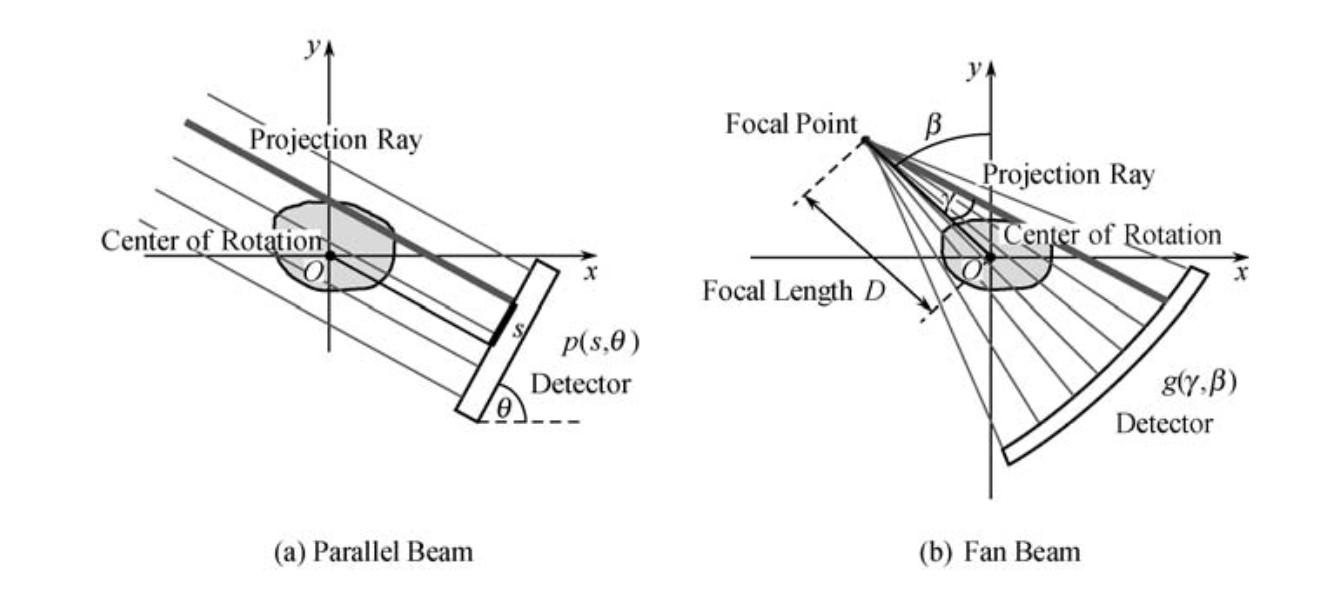
\includegraphics[width=0.3\textwidth]{images/PvsB.jpg}
\caption{Parallel Beams and Fan Beams \cite{zeng2017image}}\label{fig:PvsB}
\end{figure}

In Figure \ref{fig:PvsB}b, the projection angle with respect to center of rotation is defined as $\beta$ and the deviation from the center beam that is parallel to the $\beta$ beam is defined as $\gamma$ angles. In addition, the source to origin distance is labelled as $D$, resulting in source to detector distance of $2D$. 

With source to detector distance redefined as D and the remaining quantities defined as above, one could transform the equation in \ref{eq:radongeneral} to \ref{eq:transformedgeneral} using Eqn. \ref{eq:trans1} and \ref{eq:trans2}.
\begin{align}
	t &= D \cdot sin(\gamma) \label{eq:trans1} \\
	\theta &= \beta + \gamma \label{eq:trans2} \\
	p_{\beta}(\gamma) &= \iint\limits_{-\infty}^{\ \ \ \infty}\mu(x,y)\delta(xcos(\theta)+ysin(\theta) \label{eq:transformedgeneral} \\&-Dsin(\gamma))d\gamma d\beta \nonumber 
\end{align}

\subsection{Algebraic Reconstruction Technique}
The idea of converting the tomography problem to a linear system of equations and solving it iteratively originates from the technique which was first introduced by Gordon \textit{et al.} in \cite{gordon1970algebraic} for solving the problem of three-dimensional reconstruction from projections in electron microscopy and radiology. The method utilizes the Kaczmarz algorithm described in \cite*{kaczmarz1993approximate} as follows:

\begin{figure}[h]
\centering
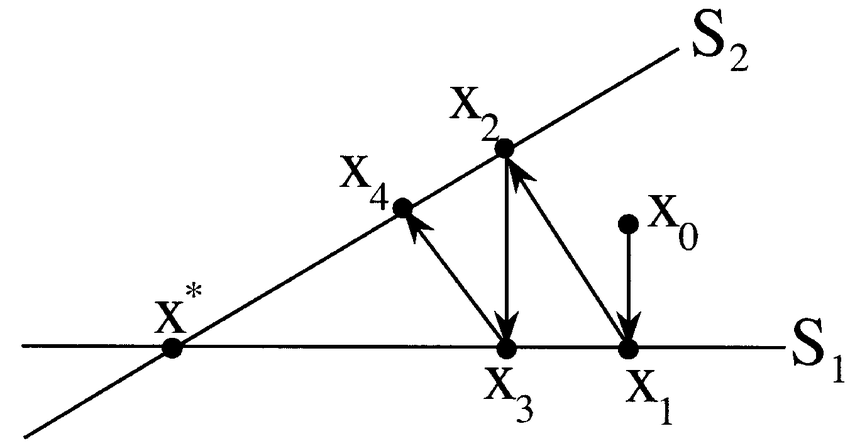
\includegraphics[width=0.3\textwidth]{images/Graphical-representation-of-the-Kaczmarzs-algorithm.png}
\caption{Kaczmarz Algorithm for solving linear systems of equations}\label{fig:kaczmarz}
\end{figure}

\begin{enumerate}
	\item Start with an initial random guess in the hyperspace of problem dimensions. 
	\item Project the solution vector onto the hyperplanes described by the rays whose parameters are determined by the line integrals taken along the corresponding ray. 
	\item Repeat the procedure until the termination condition is satisfied. This can be chosen as an error rate or number of iterations.  
\end{enumerate}

These steps can be summarized in the following update equation: 

\begin{equation}
	f^{(k+1)} = f^{(k)} - \alpha\frac{(f^Tw_j - p_j)}{||w||} 
\end{equation}

where f is the flattened image, $\alpha$ is the relaxation parameter, $w_j$ is the weights of the hyperplane defined by the $j_{th}$ ray and $p_j$ is the projection value of the corresponding ray. 
\\
\\
However, images reconstructed with this procedure exhibit a very noisy salt and pepper characteristic. To decrease the effect of this behavior without the changing the algorithm, one can optimize the order of selection of rays so that the projections hyperplanes are far from each other. This resulting in better quality pixel updates hence improves the convergence of the algorithm.

\subsection{Sequential Iterative Reconstruction Technique}

It is known that there is no single point intersections in the ART hyperplanes when the projections are corrupted by Poisson noise \cite*{dong2020accelerated}.  
In 1970, Gilbert \textit{et al.} in \cite*{gilbert1972iterative} proposed SIRT algorithm to overcome this effect by applying the computed pixel updates simultaneously, rather than equation by equation. 

In SIRT, the system $Ax=b$ where A is the projection matrix, is solved by minimizing the $\mathcal{L_2}$ norm cost function $$J = ||Ax-b||_2^2$$
Using gradient descent, the update formula becomes:
\begin{equation}
	f^{(k+1)} = f^{(k)} - \alpha A^T(Ax^{(k)}-b)
\end{equation}

The authors of \cite*{dong2020accelerated} states that for $0<\alpha<\frac{2}{||A^TA||}$, the convergence of the algorithm is guaranteed. 

\subsection{Simultaneous Algebraic Reconstruction Technique}

Although SIRT exhibits a good performance when it is compared to ART, it requires much higher iterations to converge. Andersen \& Kak proposes a new method to estimate the overall image in fewer iterations by introducing a new pixel basis to the forward problem in \cite*{andersen1984sart}. The algorithm composes of the following steps:
\begin{enumerate}
	\item A circular reconstruction region inside the image is determined. 
	\item The crossing segment of the rays with reconstruction region is divided into $M$ equidistant points.
	\item The value of the continuous distribution of the image $\hat{f}$ is calculated by using the square-pyramid shaped bilinear elements with a support of 4 pixels.
	\item The projections are found as the integrations of the image estimates along that line. 
\end{enumerate}

\section{Implementation} \label{sec:implementation}

In this section, the computer implementation of the scientific background explained in Section \nameref{sec:theory} is going to be described.

\subsection{Projection}
\begin{algorithm}[h]
\caption{Projection algorithm}
\begin{algorithmic}
\Procedure{PROJECTIONS}{$I,N_D, L_D, L_{SD}$} 
   \For{Projection angle $\beta$}
		 \For{Fan beam angle $\gamma$}
		\State Calculate x intersection
		\State Calculate y intersection
		\State Sort \Comment{Regular grid}
		\State Find distance between intersections \Comment{weights}
		\State Find the corresponding pixels
		\State Calculate projection \Comment{$weights \cdot I(pixels)$}
		\State Store in projection matrix
	  \EndFor
   \EndFor
   \State \textbf{return Projection matrix}
\EndProcedure
\label{alg:projection}
\end{algorithmic}
\end{algorithm}

\newpage
\subsection{Reconstruction}

\begin{algorithm}[h]
	\caption{ART Algorithm}
	\begin{algorithmic}
		\Procedure{ART}{$PROJECTIONS,N_D, L_D, L_{SD}$} 
		\State Get the angle step size from Projections. 
		\State Get the number of the beams from Projections. 
		\State Set initial random guess $f^{(0)}$
		   \For{Projection angle $\beta$}
				 \For{Fan beam angle $\gamma$}\\
				\Comment{$Line = F(x,y,\beta,\gamma)$}
				\State Iteratively project the current solution on one of the hyperplanes defined by the ray equations.
				\State Check the convergence to continue optimization.
			  \EndFor
		   \EndFor
		   \State Reshape the solution vector to image. 
		   \State \textbf{return IMAGE}
		\EndProcedure
	\label{alg:ART}
	\end{algorithmic}
\end{algorithm}

\begin{algorithm}[h]
	\caption{SIRT Algorithm}
	\begin{algorithmic}
		\Procedure{ART}{$PROJECTIONS,N_D, L_D, L_{SD}$} 
		\State Allocate projection matrix in sparse form.
		\State Get the angle step size from Projections. 
		\State Get the number of the beams from Projections. 
		\State Set initial random guess $f^{(0)}$
		   \For{Projection angle $\beta$}
				\For{Fan beam angle $\gamma$}
				\State Determine the weights corresponding to the current beam and the corresponding pixels.
				\State Place the weight vector into the matrix.
			  \EndFor
		   \EndFor
		   \For{iteration $n$}
				\State $f^{(k+1)} = f^{(k)} - \alpha A^T(Ax^{(k)}-b)$
		   \EndFor
		   \State Reshape the solution vector $f$ to image. 
		   \State \textbf{return IMAGE}
		\EndProcedure
	\label{alg:SIRT}
	\end{algorithmic}
\end{algorithm}

\begin{algorithm}[h]
	\caption{SART Algorithm}
	\begin{algorithmic}
		\Procedure{ART}{$PROJECTIONS,N_D, L_D, L_{SD}$} 
		\State Allocate projection matrix in sparse form.
		\State Get the angle step size from Projections. 
		\State Get the number of the beams from Projections. 
		\State Set initial random guess $f^{(0)}$
		   \For{Projection angle $\beta$}
				\For{Fan beam angle $\gamma$}
				\State Segment the line into $M$ equidistant vectors. 
				\State Find the distance $\Delta s$ between the consecutive points.
				\For{each pixel in the image}
					\State{Calculate the contribution $d_{ijm}$ to the $m^{th}$ point on the segment in terms of bilinear interpolation weights}
					\State {$a_{ij} = \sum d_{ijm}\Delta s$}
				\EndFor 
			  \EndFor
		   \EndFor
		   \For{iteration $n$}
				\State $f^{(k+1)} = f^{(k)} - \alpha A^T(Ax^{(k)}-b)$
		   \EndFor
		   \State Reshape the solution vector $f$ to image. 
		   \State \textbf{return IMAGE}
		\EndProcedure
	\label{alg:SART}
	\end{algorithmic}
\end{algorithm}

\newpage

The developed application implements the above algorithms in order to project and reconstruct the image. All components of the software and the Graphical User Interface is implemented in MATLAB(The MathWorks\textsuperscript{\textregistered}, Inc., Natick, Massachusetts, United States.) The guide to how to use the graphical user interface can be achieved in the README section of the following repository: \href{https://github.com/kutay-ugurlu/Fan-Beam-CT-ART-Simulation}{github.com/kutay-ugurlu/Fan-Beam-CT-ART-Simulation}.

\subsection{Early Stopping}
Since these algorithms use heuristic approaches or local optimizers, error metrics can diverge in some situations. To overcome this problem, an early stopping script is developed. This program keeps track of the current cumulated error vector that contains error metrics for previous iterations and takes an input called \textbf{patience}, which describes the number of iterations to wait for the algorithm to reduce the error in the next iteration. When this patience limit is achieved, algorithm outputs the reconstruction having the minimum relative error defined in Eqn. \ref{eq:relativeerror}, where $\hat{x}$ represents the reconstructed image and $x$ represents the ground truth.  

\begin{equation}
	Relative Error = \frac{||\hat{x} - x||}{||x||}
\end{equation}

\newpage

\section{Results}\label{sec:results}

\begin{figure}[h]
	\centering
	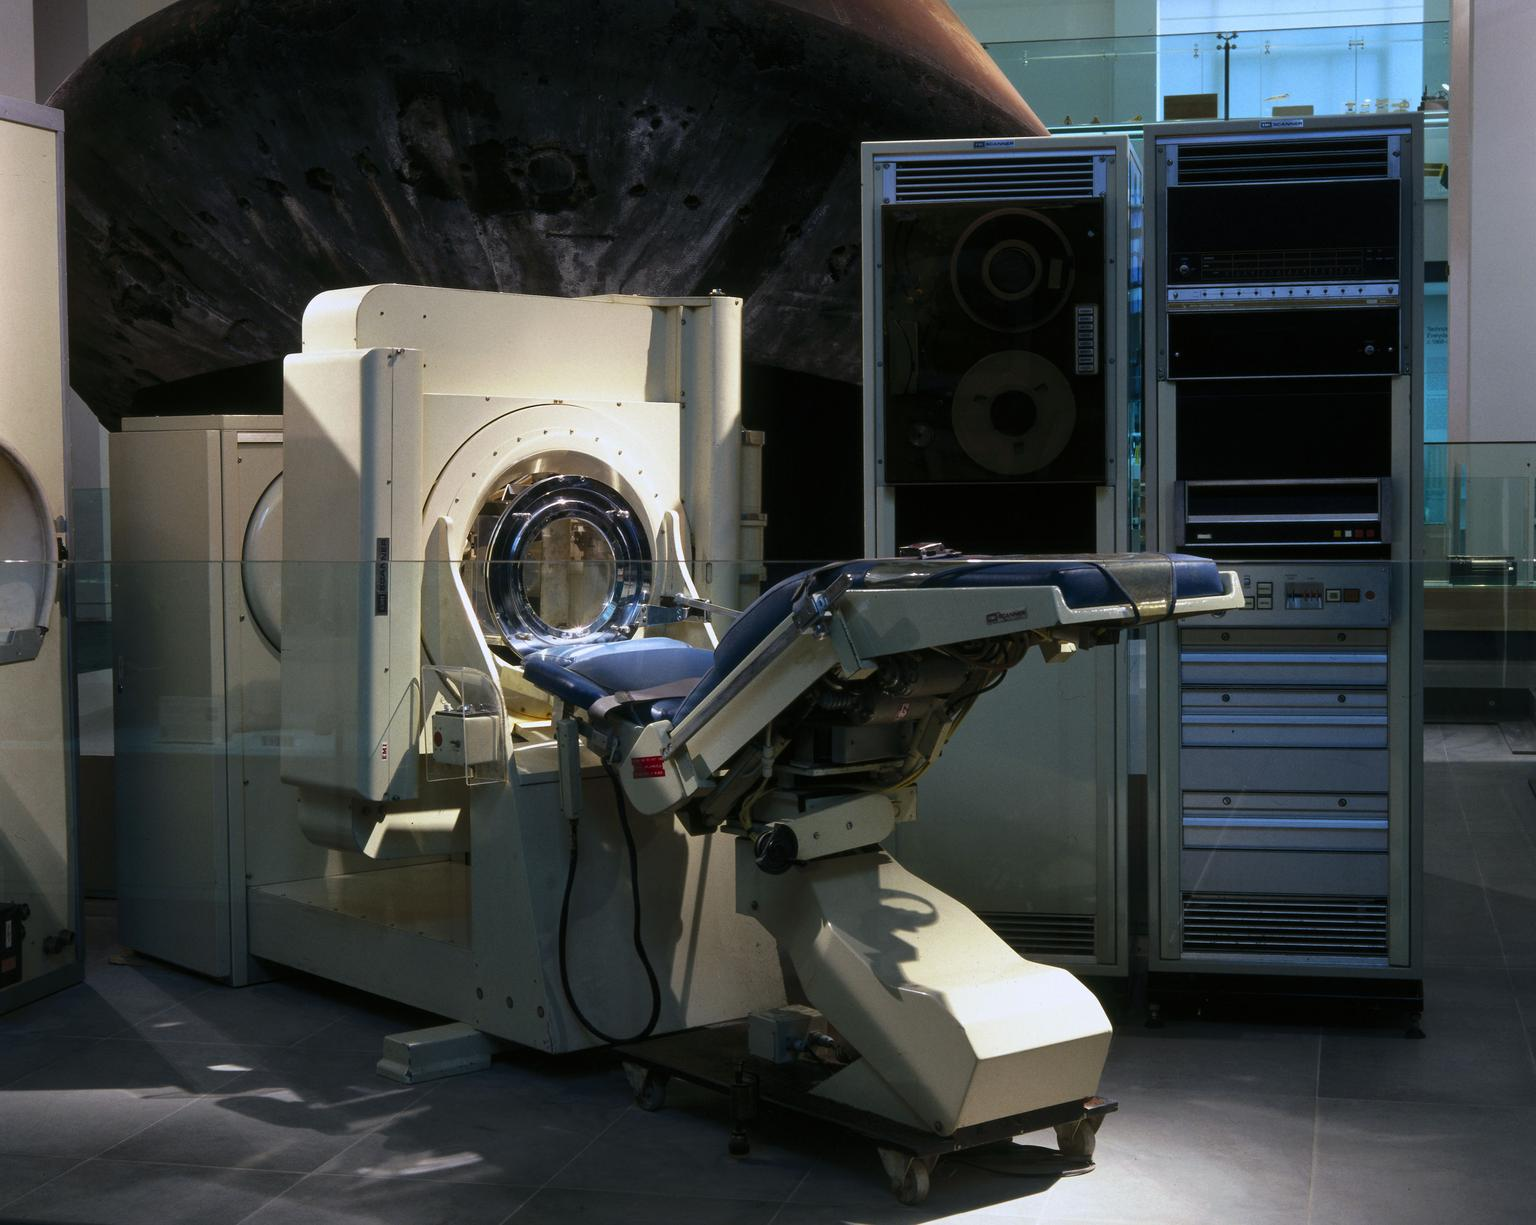
\includegraphics[width=0.4\textwidth, height=0.2\textwidth]{images/CT.jpg}
	\caption{First EMI Scanner \cite{emict}}\label{fig:CT1010}
\end{figure}
\begin{figure}[h]
	\centering
	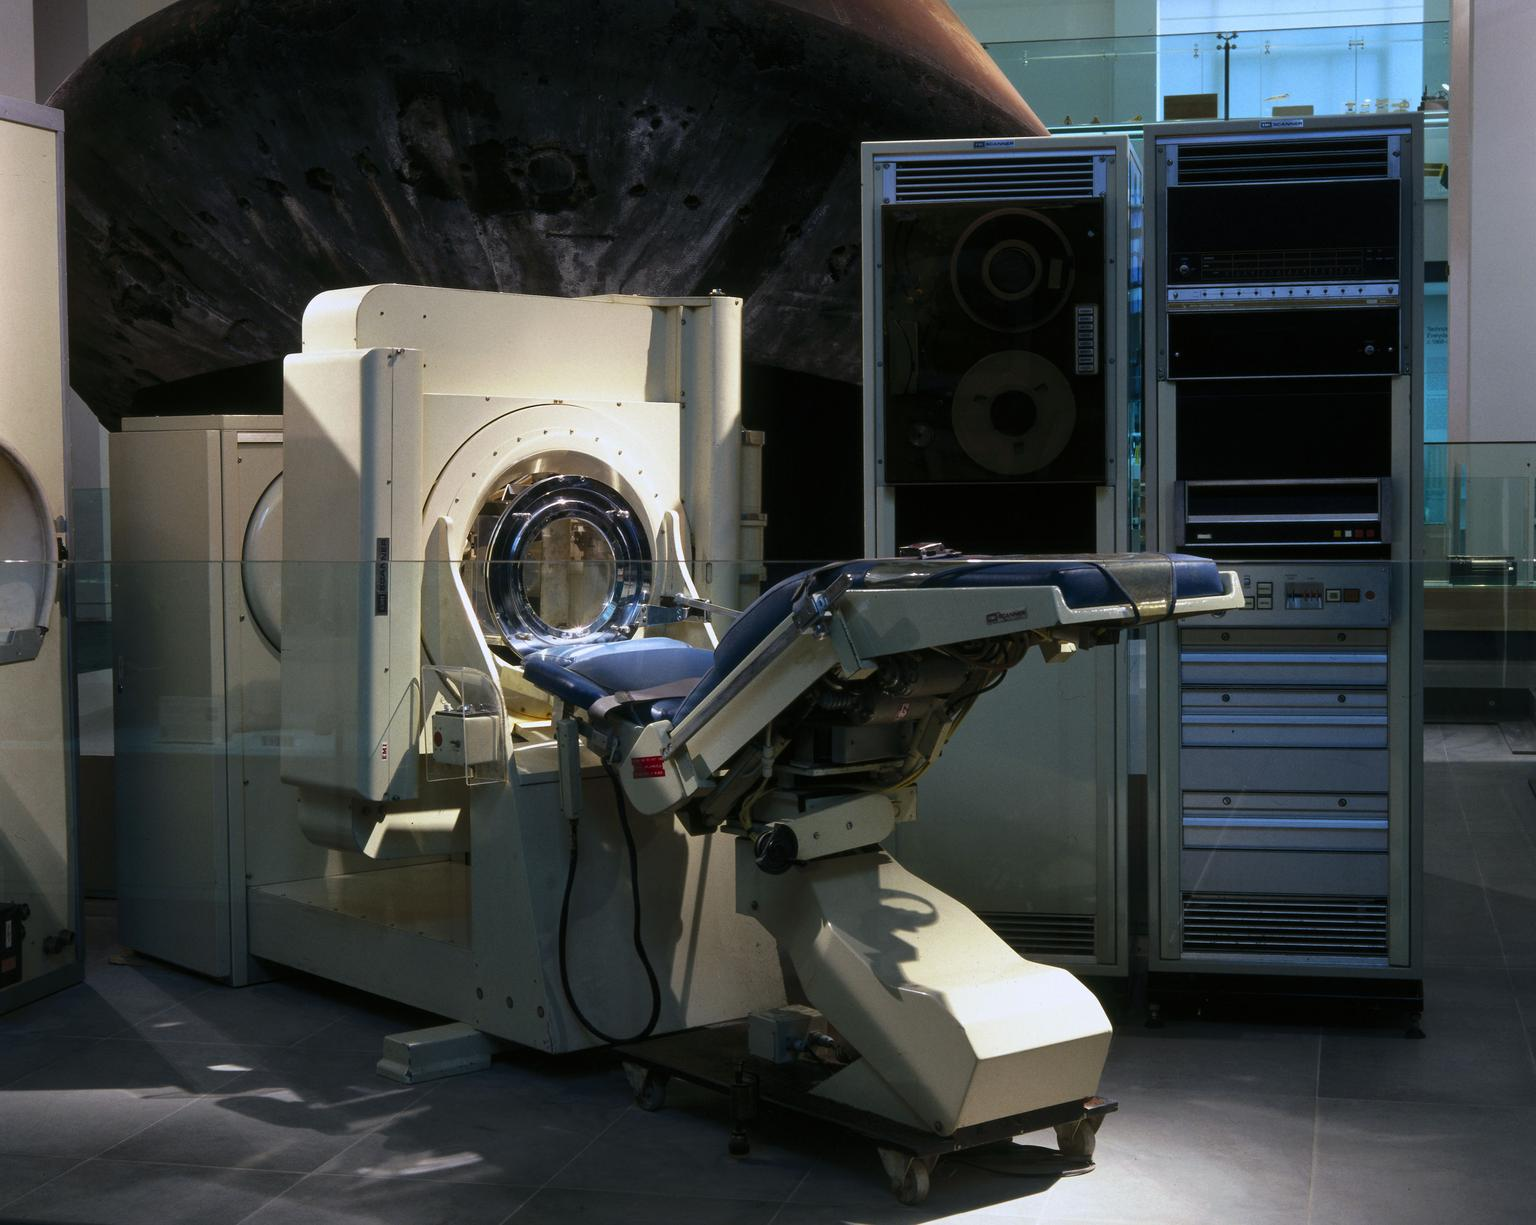
\includegraphics[width=0.4\textwidth, height=0.2\textwidth]{images/CT.jpg}
	\caption{First EMI Scanner \cite{emict}}\label{fig:CT1010}
\end{figure}
\begin{figure}[h]
	\centering
	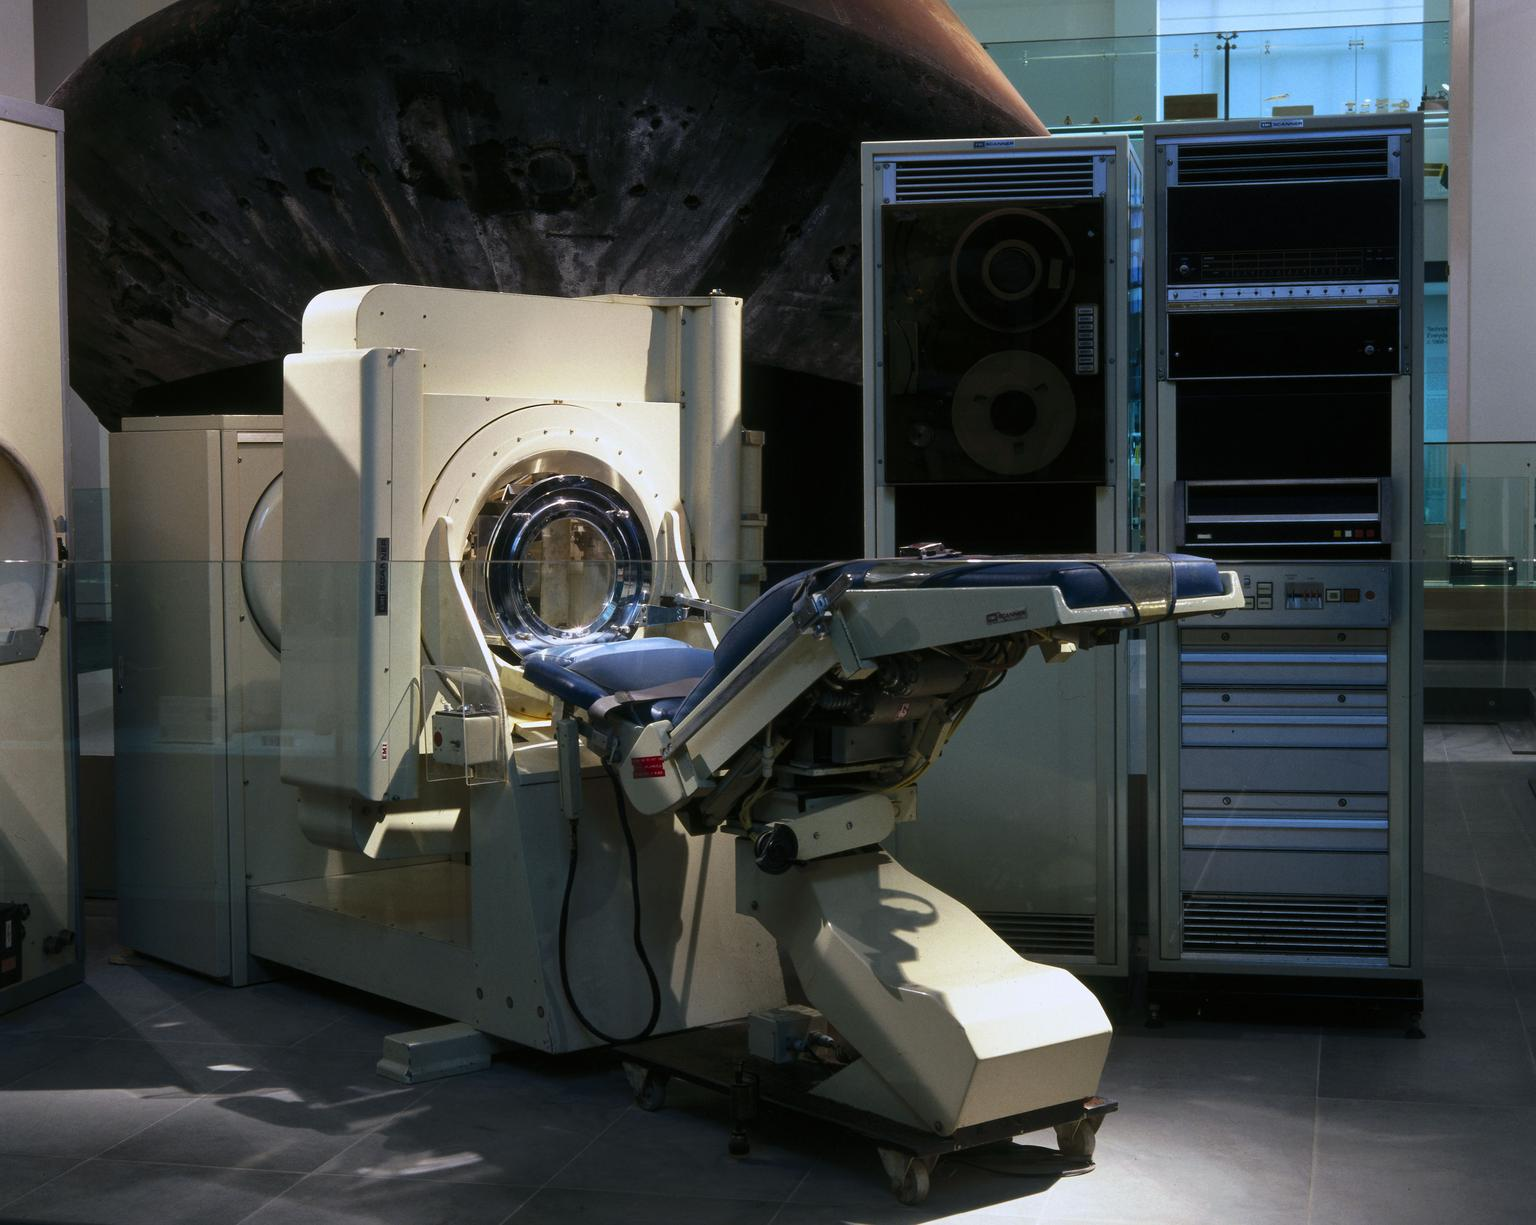
\includegraphics[width=0.4\textwidth, height=0.2\textwidth]{images/CT.jpg}
	\caption{First EMI Scanner \cite{emict}}\label{fig:CT1010}
\end{figure}

\newpage
\printbibliography
\end{document}
